\documentclass{article}
\usepackage{graphicx} % Required for inserting images
\usepackage{tikz}
\usetikzlibrary{matrix}

\title{Credit Card Fraud Detection using various Machine Learning techniques}
\author{Konstantinos Baktalias}
\date{November 2023}

\begin{document}

\maketitle

\begin{abstract}
    The undertaken endeavour examines various classical machine learning methodologies, including support vector machines, k-nearest neighbours, and logistic regression. The primary objective is the identification of fraudulent transactions, employing both individual techniques and combinations thereof. The foundation of this investigation lies in Kaggle's Credit Card Fraud Detection dataset. The accompanying report incorporates the code utilized throughout this study, and it is noteworthy that each method and model has been meticulously implemented from the ground up.
\end{abstract}

\section{Data Pre-processing}

Upon examining the given dataset, it becomes evident that the count of non-fraudulent transactions significantly surpasses that of fraudulent transactions. This poses a significant challenge, as a machine learning model is prone to exhibit a pronounced bias toward non-fraudulent transactions, potentially resulting in an unreliable classifier. To mitigate this issue, it is imperative to address the imbalance by generating synthetic data.

Creating synthetic data to account for the disparity between non-fraudulent and fraudulent transactions and subsequently integrating this synthetic data with the original fraudulent transactions dataset appears to be a viable approach. Nevertheless, it is imperative to establish criteria for generating this data that ensures mitigation of information discrepancies. As per our understanding derived from the Law of Large Numbers, for a sequence of independent and identically distributed random variables $X_1, X_2, ...,X_n$ with mean $\mu$ and variance $\sigma ^2$, we know that $$\lim_{n \rightarrow \infty} P(|\frac{X_1+X_2+ ...+X_n}{n} - \mu|\ge \epsilon)=0$$, where $\epsilon$ is any positive number.

We aim for our model to generalise around the mean of feature vectors. To achieve this, we calculate the mean value $\mu_i$ and standard deviation $\sigma_i$ for each feature $i$, and subsequently generate new feature values following a normal distribution $\mathcal{N}(x|\mu_i, \sigma_i)$. This approach results in our classifiers being trained on a broader range of fraudulent transactions due to the increased variance introduced during the feature generation process.

\section{Logistic Regression}
Logistic regression proves to be an effective algorithm for addressing binary classification problems. The model comprises parameters, including a weight vector $\textbf{w}$ corresponding to each feature and a bias term $w_0$. To make predictions for an input vector $\textbf{x}$, the model computes the result of the operation $z = \textbf{w}^{T}\textbf{x} + w_0$ and passes it through the sigmoid activation function, resulting in the value $a$.
$$a=\sigma(z)=\frac{1}{1+exp(-z)}$$ Following the sigmoid activation, the decision is made: if $a \ge 0.5$, the associated feature vector is classified as class $1$; otherwise, it is classified as class $0$.

The training procedure for a logistic regression model, where the output for a given feature vector $\textbf{x}$ is denoted as $h(\textbf{x})$, focuses on maximizing the log-likelihood function $\ell(h)$. The log-likelihood is defined as $$\ell(h) = -\sum^{N}_{i=1} y_i \ln[h(\textbf{x}_i)] + (1 - y_i) \ln[1 - h(\textbf{x}_i)]$$In this particular context, the maximization process is accomplished by employing Stochastic Gradient Descent on each training sample.

After conducting $k$-fold cross-validation on the provided dataset with $k=5$, the model demonstrates an overall accuracy of $\sim 0.78$. While this performance may initially appear satisfactory, it is found to be comparatively subpar when contrasted with later encountered methods. To gain a more comprehensive insight, we derive the average confusion matrix by repeating the $k$-fold cross-validation process with $k=5$.
\begin{center}
    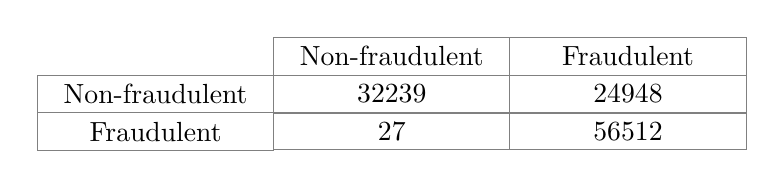
\begin{tikzpicture}
        \matrix[matrix of nodes, nodes={draw=gray, anchor=center, minimum width=3cm}, column sep=-\pgflinewidth, row sep=-\pgflinewidth] (A) {
             & Non-fraudulent & Fraudulent \\
            Non-fraudulent & 32239 & 24948 \\
            Fraudulent & 27 & 56512 \\
        };
    \end{tikzpicture}
\end{center}
It is evident that the model has a noticeable inclination to incorrectly classify a higher number of non-fraudulent transactions as fraudulent compared to the other way around. This suggests a distinct bias towards classifying transactions as fraudulent.
\\
\\

\section{K Nearest Neighbours}
The K Nearest Neighbors method is a viable option for addressing this problem. Essentially, the classification procedure involves identifying the $k$, nearest points, in other words, those with the smallest distances, in the feature space of the dataset. Subsequently, the prediction is determined by the class with the highest frequency among these $k$ data points.

To enhance prediction efficiency, the model is structured as a kd-tree. Employing simpler techniques such as brute force would prove notably inefficient. The process of finding the $k$ nearest neighbours in a kd-tree operates with a time complexity of $\mathcal{O}(\log(n) + k)$, where $n$ represents the number of training data samples used in constructing the tree.

Concerning the performance metrics obtained through $k$-fold cross-validation on the given dataset with five folds for $k=5$ K Nearest Neighbors instance, the model exhibits an overall accuracy of  $\sim 0.94$. The average confusion matrix is 
\begin{center}
    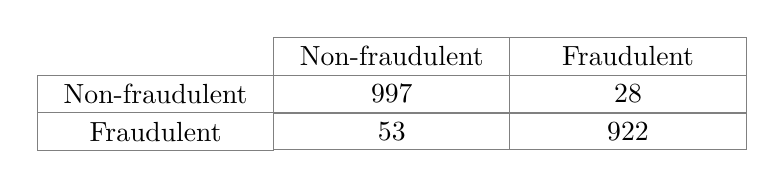
\begin{tikzpicture}
        \matrix[matrix of nodes, nodes={draw=gray, anchor=center, minimum width=3cm}, column sep=-\pgflinewidth, row sep=-\pgflinewidth] (A) {
             & Non-fraudulent & Fraudulent \\
            Non-fraudulent & 997 & 28 \\
            Fraudulent & 53 & 922 \\
        };
    \end{tikzpicture}
\end{center}
Notably better than logistic regression.

\section{Support Vector Machine}

Support Vector Machines work intuitively by finding the optimal hyperplane that best separates different classes in a dataset. The basic idea is to identify a hyperplane that maximizes the margin between data points of different classes. The margin is the distance between the hyperplane and the nearest data points from each class. The data points that are closest to the hyperplane and influence the position and orientation of the hyperplane are called support vectors. 

Most often, data does not exhibit perfect linear separability, prompting the introduction of a relaxation factor denoted as $C$.

The hyperparameters of the model include a weight vector $\textbf{w}$ associated with each feature, a bias term $w_0$, and the relaxation factor $C$.

In a more mathematical context, the model's output is determined by conditions: if $\textbf{w}^T\textbf{x}_i+w_0\ge 1$, the model predicts $1$, and if $\textbf{w}^T\textbf{x}_i+w_0\le -1$, it predicts $-1$.

The objective of the optimization process is to minimize the expression $$\min_{\textbf{w}, w_0}\frac{1}{2}||\textbf{w}||^2 + C\sum^{N}_{i=1}[1 - y_i(\textbf{w}^T\textbf{x} + w_0)]_{+}$$.

Regarding the performance metrics derived from $k$-fold cross-validation on the provided dataset with $k=5$, the model exhibits an overall accuracy of  $\sim 0.98$, and the corresponding confusion matrix is as follows:

\begin{center}
    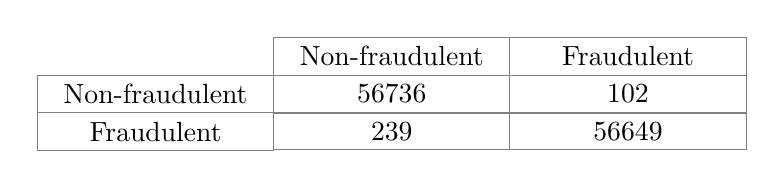
\begin{tikzpicture}
        \matrix[matrix of nodes, nodes={draw=gray, anchor=center, minimum width=3cm}, column sep=-\pgflinewidth, row sep=-\pgflinewidth] (A) {
             & Non-fraudulent & Fraudulent \\
            Non-fraudulent & 56736 & 102 \\
            Fraudulent & 239 & 56649 \\
        };
    \end{tikzpicture}
\end{center}
The best performance encountered thus far.

\section{Multi-model Majority Vote}
The main motivation Condorcet's Jury Theorem which states ```If $p>0.5$, adding voters to the jury increases the probability of a correct majority vote, assuming votes are independent.```. This forms a foundation for constructing models that take various features into account, where certain models may excel at classifying specific features. It also facilitates the creation of random models, which are combinations of models considering features randomly, eliminating the need for manual configuration. Generating a substantial number of models, however, becomes computationally expensive. Distributing the task of model generation is advisable. In a limited set of model generations, the best random model achieved an overall accuracy of  $\sim 0.96$, slightly inferior to the performance of the support vector machine.

\section{Concluding remarks}
The support vector machine, when considering all features, appears to outperform all other methods. However, it is noteworthy that randomly generating models has the potential to surpass the performance of the support vector machine after generating a substantial number of models.

\end{document}
